\documentclass[uplatex,dvipdfmx,a4paper,11pt]{jsarticle}

\usepackage{docmute}


% 数式
\usepackage{amsmath,amsthm,amssymb}
\usepackage{bm}
% 画像
\usepackage{graphicx}

\usepackage{multirow}
\usepackage{wrapfig}
\usepackage{ascmac}
\usepackage{xcolor}


\usepackage{makeidx}
\makeindex

\graphicspath{{../../_Figures//}{../../_Figures/Rheology/}}

\usepackage{qrcode}
\setlength\lineskiplimit{0pt}
\setlength\normallineskiplimit{0pt}

\usepackage{qexam}

\usepackage{titlesec}
\titleformat*{\section}{\Large\bfseries}
\titleformat*{\subsection}{\large\bfseries}
\titleformat*{\subsubsection}{\normalsize\bfseries}
\titleformat*{\paragraph}{\normalsize\bfseries}

% ページ設定
% \pagestyle{empty}
% 高さの設定
\setlength{\textheight}{\paperheight}   % ひとまず紙面を本文領域に
\setlength{\topmargin}{-5.4truemm}      % 上の余白を20mm(=1inch-5.4mm)に
\addtolength{\topmargin}{-\headheight}  % 
\addtolength{\topmargin}{-\headsep}     % ヘッダの分だけ本文領域を移動させる
\addtolength{\textheight}{-40truemm}    % 下の余白も20mmに%% 幅の設定
\setlength{\textwidth}{\paperwidth}     % ひとまず紙面を本文領域に
\setlength{\oddsidemargin}{-5.4truemm}  % 左の余白を20mm(=1inch-5.4mm)に
\setlength{\evensidemargin}{-5.4truemm} % 
\addtolength{\textwidth}{-40truemm}     % 右の余白も20mmに
% 図と本文との間
%\abovecaptionskip=-5pt
%\belowcaptionskip=-5pt
%
% 全体の行間調整
% \renewcommand{\baselinestretch}{1.0} 
% 図と表
%\renewcommand{\figurename}{Fig.}
%\renewcommand{\tablename}{Tab.}
%

% \makeatletter 
% \def\section{\@startsection {section}{1}{\z@}{1.5 ex plus 2ex minus -.2ex}{0.5 ex plus .2ex}{\large\bf}}
% \def\subsection{\@startsection{subsection}{2}{\z@}{0.2\Cvs \@plus.5\Cdp \@minus.2\Cdp}{0.1\Cvs \@plus.3\Cdp}{\reset@font\normalsize\bfseries}}
% \makeatother 

\usepackage[dvipdfmx,%
 bookmarks=true,%
 bookmarksnumbered=true,%
 colorlinks=false,%
 setpagesize=false,%
 pdftitle={数式に頼らない直感的理解による材料設計のためのレオロジー⼊⾨},%
 pdfauthor={佐々木裕},%
 pdfsubject={},%
 pdfkeywords={レオロジー; 材料設計; }]{hyperref}
\usepackage{pxjahyper}

\usepackage{plext}

\usepackage{niceframe} 
\usepackage{framed}
\newenvironment{longartdeco}{%
  \def\FrameCommand{\fboxsep=\FrameSep \artdecoframe}%
  \MakeFramed {\FrameRestore}}%
 {\endMakeFramed}
 
\usepackage{siunitx}

\newcommand{\rmd}{\mathrm{d}}

\usepackage[inline]{showlabels}

\begin{document}

\question{演習問題 1}
内容を振り返るために、以下に示した文章例の中から適切な記述のものを複数選んでください。
\begin{qlist}
	\qitem 物質の三態についての、正しい言葉はどれでしょうか?
		\begin{qlist2}
			\qitem マクロな視点で考えると、気体と液体は流れますが、固体は流れなくて形状を変えません。
			\qitem 固体は、何らかの粒子が規則的に並んだ「結晶」としてモデル化される場合が多く見受けられます。
			\qitem 固体の粒子間隔は、一般に液体のそれよりも長くなっています。
			\qitem 液体をミクロに見ても、内部には一見してわかるような規則的な構造を有しません。
			\qitem 気体において粒子は自由に運動していますが、その粒子間隔は液体よりも短くなっています。
		\end{qlist2}
        \vspace{3mm}
        \begin{itembox}[l]{解答}
            (正しい選択肢)\\
            (a), (b), (d)\\
            (解説)\\
            固体のモデルである結晶においては一般に粒子間隔が短く、液体では気体の粒子間隔は長くなっています。
            なお、粒子間隔は密度の逆数です。

            液体をミクロに見ても、内部には一見してわかるような規則的な構造を持たないことに注意してください。
        \end{itembox}
	\qitem 結晶についての、正しい言葉はどれでしょうか?
		\begin{qlist2}
			\qitem 固体をミクロに見たとき、内部の粒子間に相互作用が存在すると考えられます。
			\qitem Lennard-Jones ポテンシャルは、相対的に速く消失する引力と遠くまで働く斥力との差として二体間の相互作用を表します。
			\qitem ポテンシャルを積分すると働く力が算出できます。
			\qitem ポテンシャルの極小値において二粒子間の力は 0 となります。
			\qitem 粒子間の距離が短くなりすぎると斥力が働き、離れすぎると引力が働きますから、その間に安定状態があります。
		\end{qlist2}
        \vspace{3mm}
        \begin{itembox}[l]{解答}
            (正しい選択肢)\\
            (a), (d), (e)\\
            (解説)\\
            Lennard-Jones ポテンシャルは、二体間の相互作用を書き表したポテンシャルです。
            これは、相対的に速く消失する斥力と遠くまで働く引力との「和」として表されていることに注意してください。
            このポテンシャルを「微分」すると、二体間に働く力が算出できます。
        \end{itembox}
	\qitem 「固体と液体」についての、正しい言葉はどれでしょうか?
		\begin{qlist2}
			\qitem 固体と液体との境目で融解や結晶化が生じるとき、比熱や体積は連続的に変化します。
			\qitem 固体の融解や液体の結晶化において、物質の内部で粒子のパッキングや運動状態も変化します。
			\qitem 液体を形成する粒子の相互の位置は、規則的では有りません。
			\qitem マクロな状態は、ミクロな粒子が熱エネルギーにより自由に動こうとするという状態と居心地のいい位置に留まりたいという状態との2つの状態のせめぎあいで決まります。
			\qitem 液体では、熱の影響が相対的に小さいので、それぞれの粒子が自由に移動します。
		\end{qlist2}	
        \vspace{3mm}
        \begin{itembox}[l]{解答}
            (正しい選択肢)\\
            (b), (c), (d)\\
            (解説)\\
            固体と液体との境目で融解や結晶化が生じるときには比熱や体積に「飛び」が生じます。
            このとき、物質の内部では粒子のパッキングや運動状態も変化していると考えられています。
            
            マクロな状態はミクロな粒子がどのように運動するかで決まり、これは、熱エネルギーとポテンシャルとの釣り合いで決まります。
            熱の影響が相対的に大きくてそれぞれの粒子が一箇所に留まらない状態が液体です。
        \end{itembox}
	\qitem 流れるということについての、正しい言葉はどれでしょうか?
		\begin{qlist2}
			\qitem 液体が流れるときには、内部の粒子が瞬間ごとの居心地のいい状態に移動しています。
			\qitem 固体と呼ばれるものは、いくら長時間待っていても決して流れません。
			\qitem 液体を速く変形すると固体的に振る舞う場合があります。
			\qitem 液体を冷却すると、結晶化するとは限らないでガラス状態になることもあります。
			\qitem ガラス化するときも、一般には体積に飛びが出てきます。
		\end{qlist2}	
        \vspace{3mm}
        \begin{itembox}[l]{解答}
            (正しい選択肢)\\
            (a), (c), (d)\\
            (解説)\\
            固体と呼ばれるものであっても、非常に長時間観察していると流れる場合もあります。
            一方、液体も固体的に振る舞うこともありますから、その境目は曖昧です。
            
            また、ガラス化してもミクロに内部を見た時には液体と見分けが付きませんから、一般に体積の飛びは有りません。
        \end{itembox}
	\qitem 応力の由来についての、正しい言葉はどれでしょうか?
		\begin{qlist2}
			\qitem 固体の応力は、内部のミクロな粒子が安定な位置から変位した結果生じると考えられます。
			\qitem 固体内部の応力は、直ちに消失します。
			\qitem 液体を変形させると、局所的に歪んだかごのような状態ができます。
			\qitem 液体においても、居心地のいい状態からの変位で応力が発生します。
			\qitem 歪んだ液体で生じた局所的な応力は、流れても消えません。
		\end{qlist2}
        \vspace{3mm}
        \begin{itembox}[l]{解答}
            (正しい選択肢)\\
            (a), (c), (d)\\
            (解説)\\
            固体内部で生じる応力はミクロな粒子の変位によるものであり、外部からの変形が維持されていれば、一般には解消されません。
            
            一方、液体で生じる局所的な応力は、ミクロな粒子の運動によるマクロな流動とともに消失します。
        \end{itembox}
\end{qlist}

\clearpage

\question{演習問題 2}
内容を振り返るために、テキストで用いた言葉を使って簡単な穴埋めを行ってください。
\begin{qlist}
	\qitem 「固体と液体」について、\qbox{(a)}から\qbox{(i)}までのカッコを埋めてください。
		\begin{qlist2}
			\qitem 粒子多体系での相互作用について
				\begin{center}
					\begin{minipage}{0.52\textwidth}
						\begin{itembox}[l]{多体系での相互作用}
							\begin{itemize}
								\item 多体の\qbox{}を簡略化して、
								\item \qbox{}の相互作用に基づくとすれば、
								\item 多体の粒子が\qbox{}の近傍で摂動
							\end{itemize}
						\end{itembox}
					\end{minipage}
					\begin{minipage}{0.32\textwidth}
						\begin{center}
						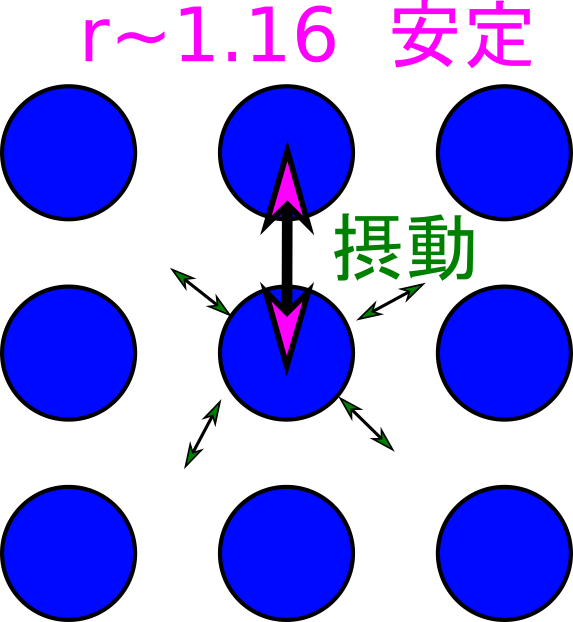
\includegraphics[width=.6\textwidth]{LJ_ryusi.png}
						\end{center}
					\end{minipage}
			\end{center}

		\qitem 固体と液体の相転移について
			\begin{center}
				\begin{minipage}{0.42\textwidth}
					\begin{itembox}[l]{固体と液体の相転移}
						\begin{itemize}
							\item マクロに見れば
							\begin{itemize}
								\item 融解、結晶時に、
								\item \qbox{}に「飛び」
							\end{itemize}
							\item ミクロに考えると、
							\begin{itemize}
								\item 内部の\qbox{}が変化
								\item \qbox{}も変化
							\end{itemize}
						\end{itemize}
					\end{itembox}
				\end{minipage}
				\begin{minipage}{0.42\textwidth}
					\begin{center}
					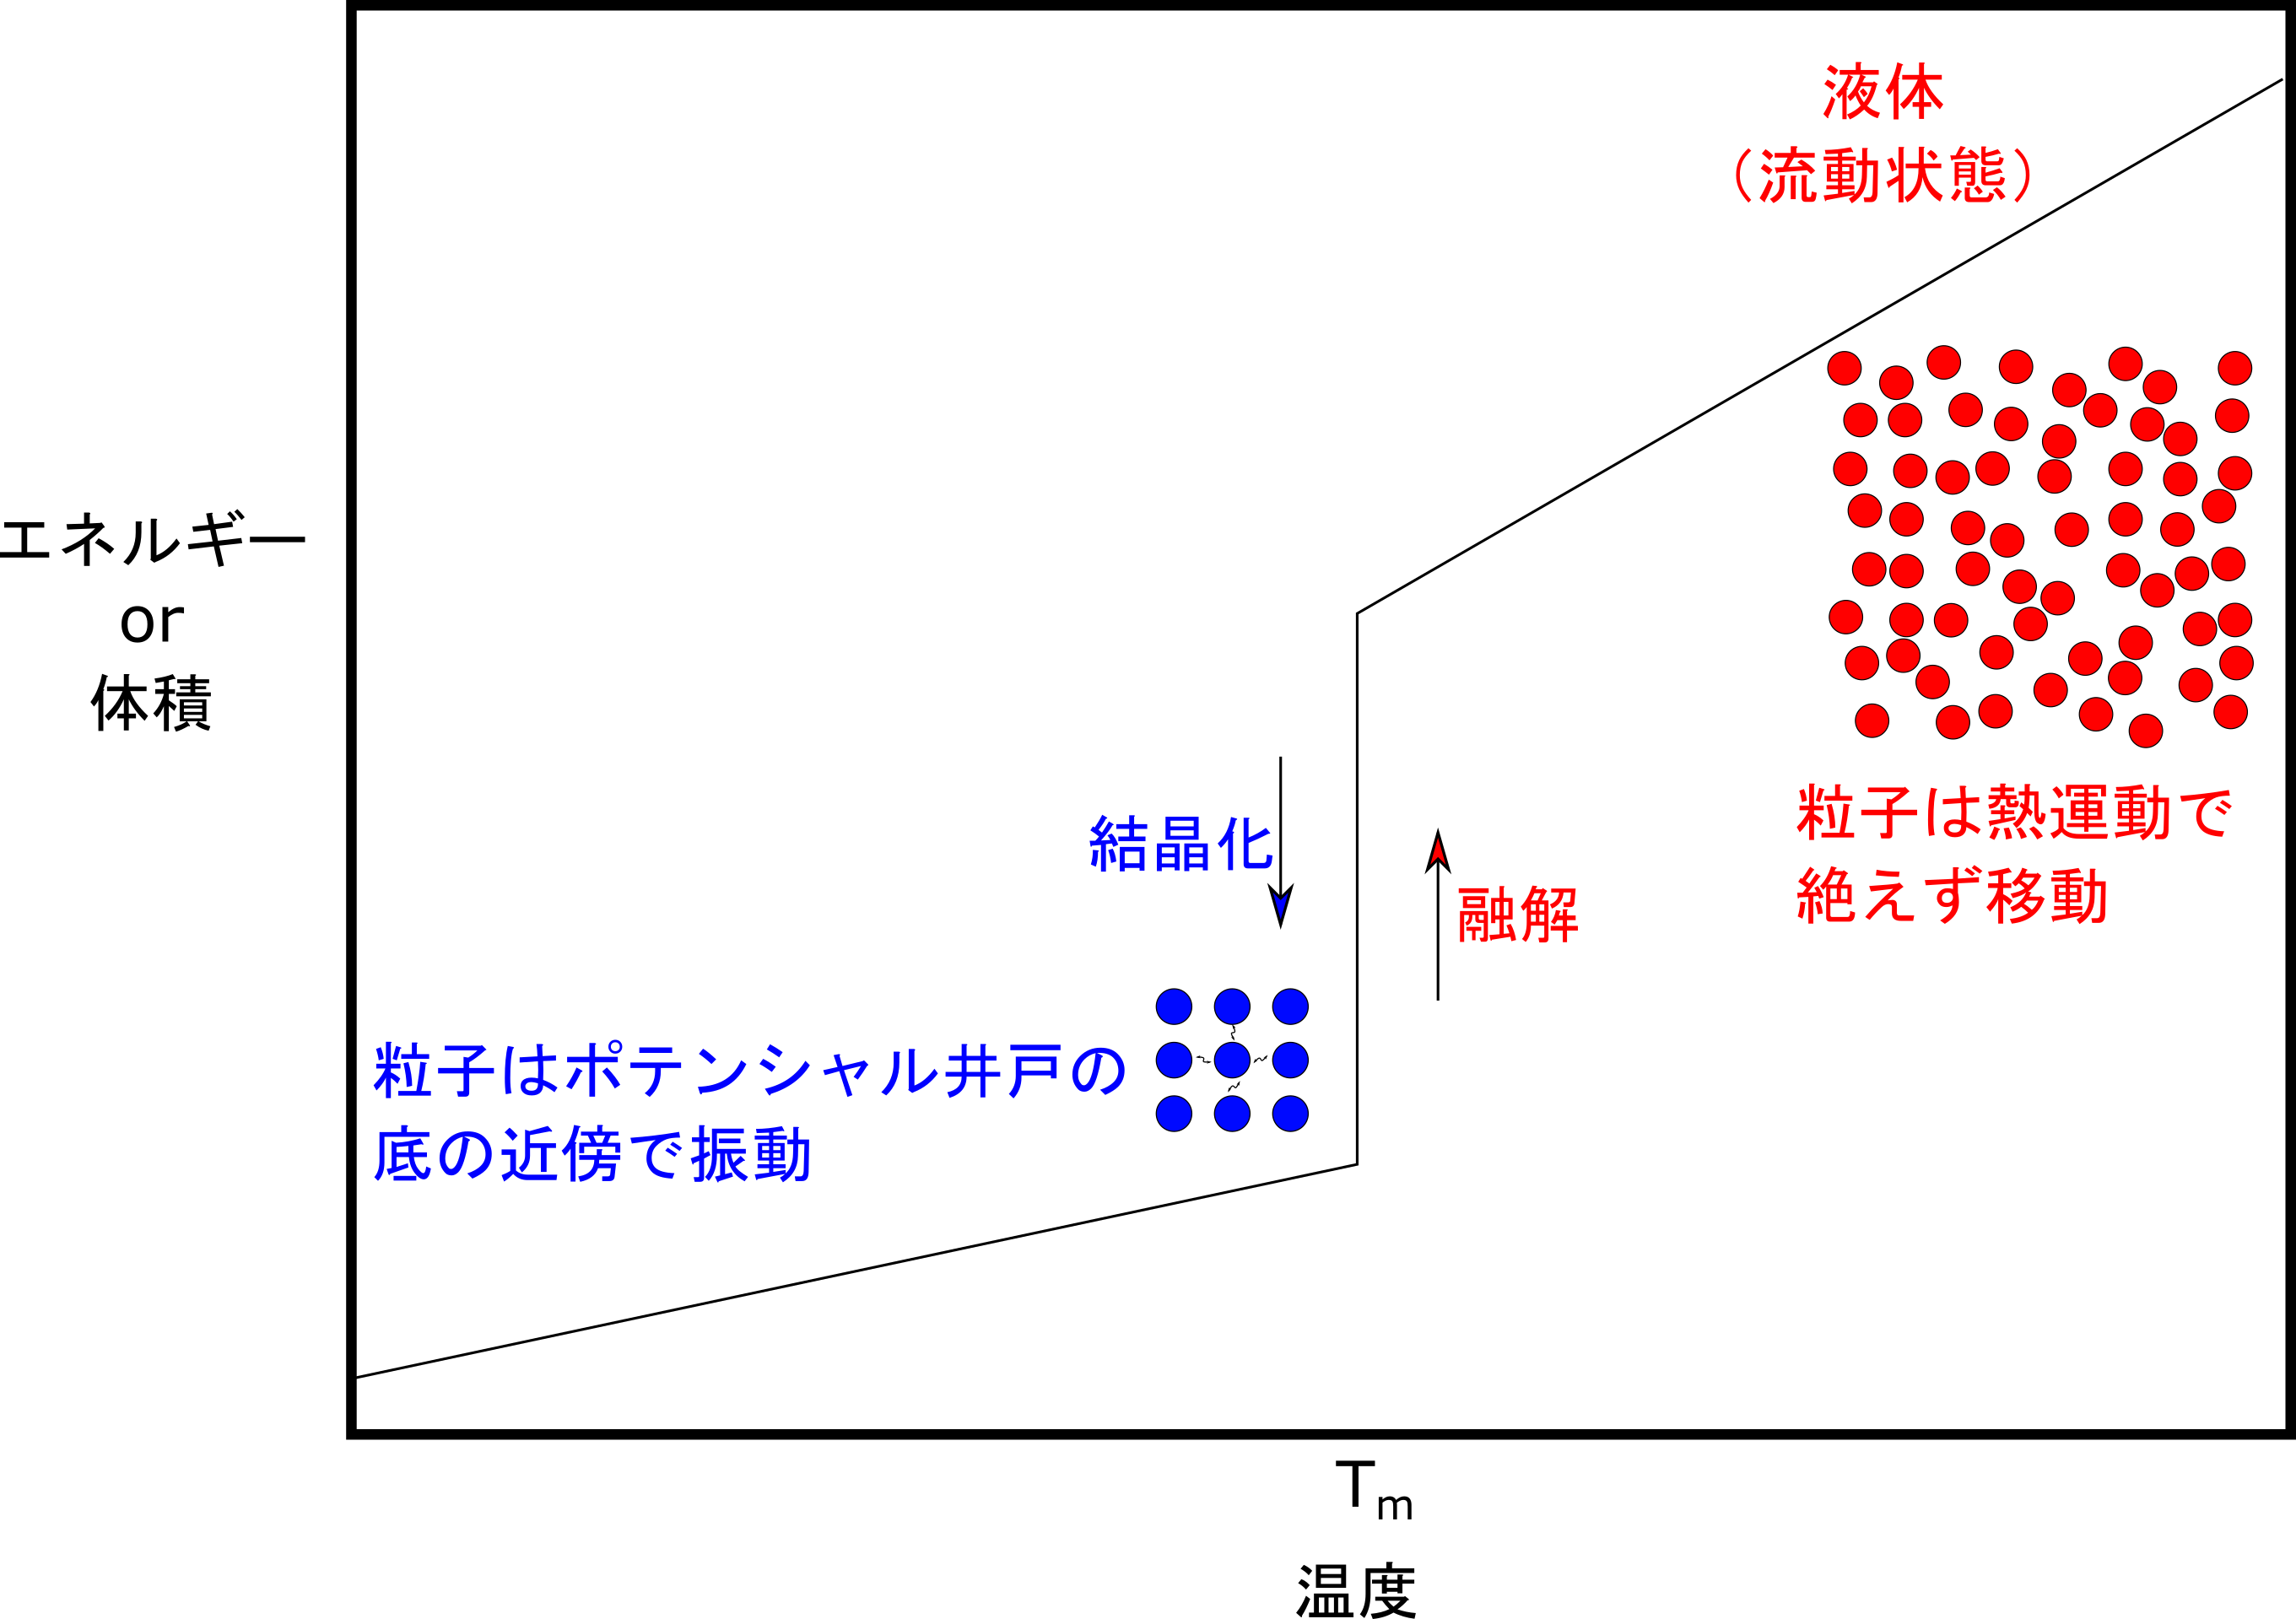
\includegraphics[width=\textwidth]{crystal_melt.png}
					\end{center}
				\end{minipage}
			\end{center}
			
			\qitem 固体と液体の違いとは
				\begin{itembox}[l]{ミクロに考えた固体と液体の違い}
					\begin{itembox}[l]{ミクロな状態での2つのせめぎあい}
						\begin{itemize}
							\item 粒子は\qbox{}で揺らされる。
							\item \qbox{}のいい位置に留まりたい。
						\end{itemize}
					\end{itembox}
					\begin{itembox}[l]{その結果として、}
						\begin{itemize}
							\item 固体:相対的に揺動小
							\begin{itemize}
								\item ポテンシャル井戸の底近傍で振動
								\item 内部構造を形成。
							\end{itemize}
							\item 液体:熱揺動が大きい
							\begin{itemize}
								\item 多くの粒子が相互作用
								\item 構造が\qbox{}
							\end{itemize}
						\end{itemize}
					\end{itembox}
				\end{itembox}

		\end{qlist2}

		\begin{itembox}[l]{選択肢}
			\begin{center}
				\begin{tabular}{lllll}
					1. 熱エネルギー	&2. 相互作用	&3. 居心地	&4. 運動状態	&5. 不定\\
					6. 二体間	&7. 比熱や体積		&8. パッキング	&9. 安定状態
				\end{tabular}
			\end{center}
		\end{itembox}
\end{qlist}

\begin{itembox}[l]{解答}
    \begin{center} 
      \begin{tabular}{|c|c|c|c|c|c|c|c|c|} \hline
        (a) & (b) & (c) & (d) & (e) & (f) & (g) & (h) & (i)\\ \hline
        2 & 6 & 9 & 7 & 8 & 4 & 1 & 3 & 5 \\ \hline		
      \end{tabular}
    \end{center}
\end{itembox}


\begin{qlist}
	\qitem 「流れるということ」について、\qbox{(j)}から\qbox{(r)}までのカッコを埋めてください。
		\begin{qlist2}
			\qitem ミクロに見た流動のイメージ
				\begin{center}
					\begin{minipage}{0.56\textwidth}
						\begin{itembox}[l]{ミクロな流動のイメージ}
							\begin{itemize}
								\item マクロな変形を与える。
								\begin{itemize}
									\item ミクロに粒子の相互位置が変化
									\item 相互のポテンシャルのために、\qbox{}粒子が発生。
									\item 粒子の移動のバランスが変化
									\item 居心地のいい位置へと\qbox{}
								\end{itemize}
								\item マクロな変形に従うように、粒子の位置が\qbox{}。
							\end{itemize}
						\end{itembox}
					\end{minipage}
					\begin{minipage}{0.3\textwidth}
						\begin{center}
						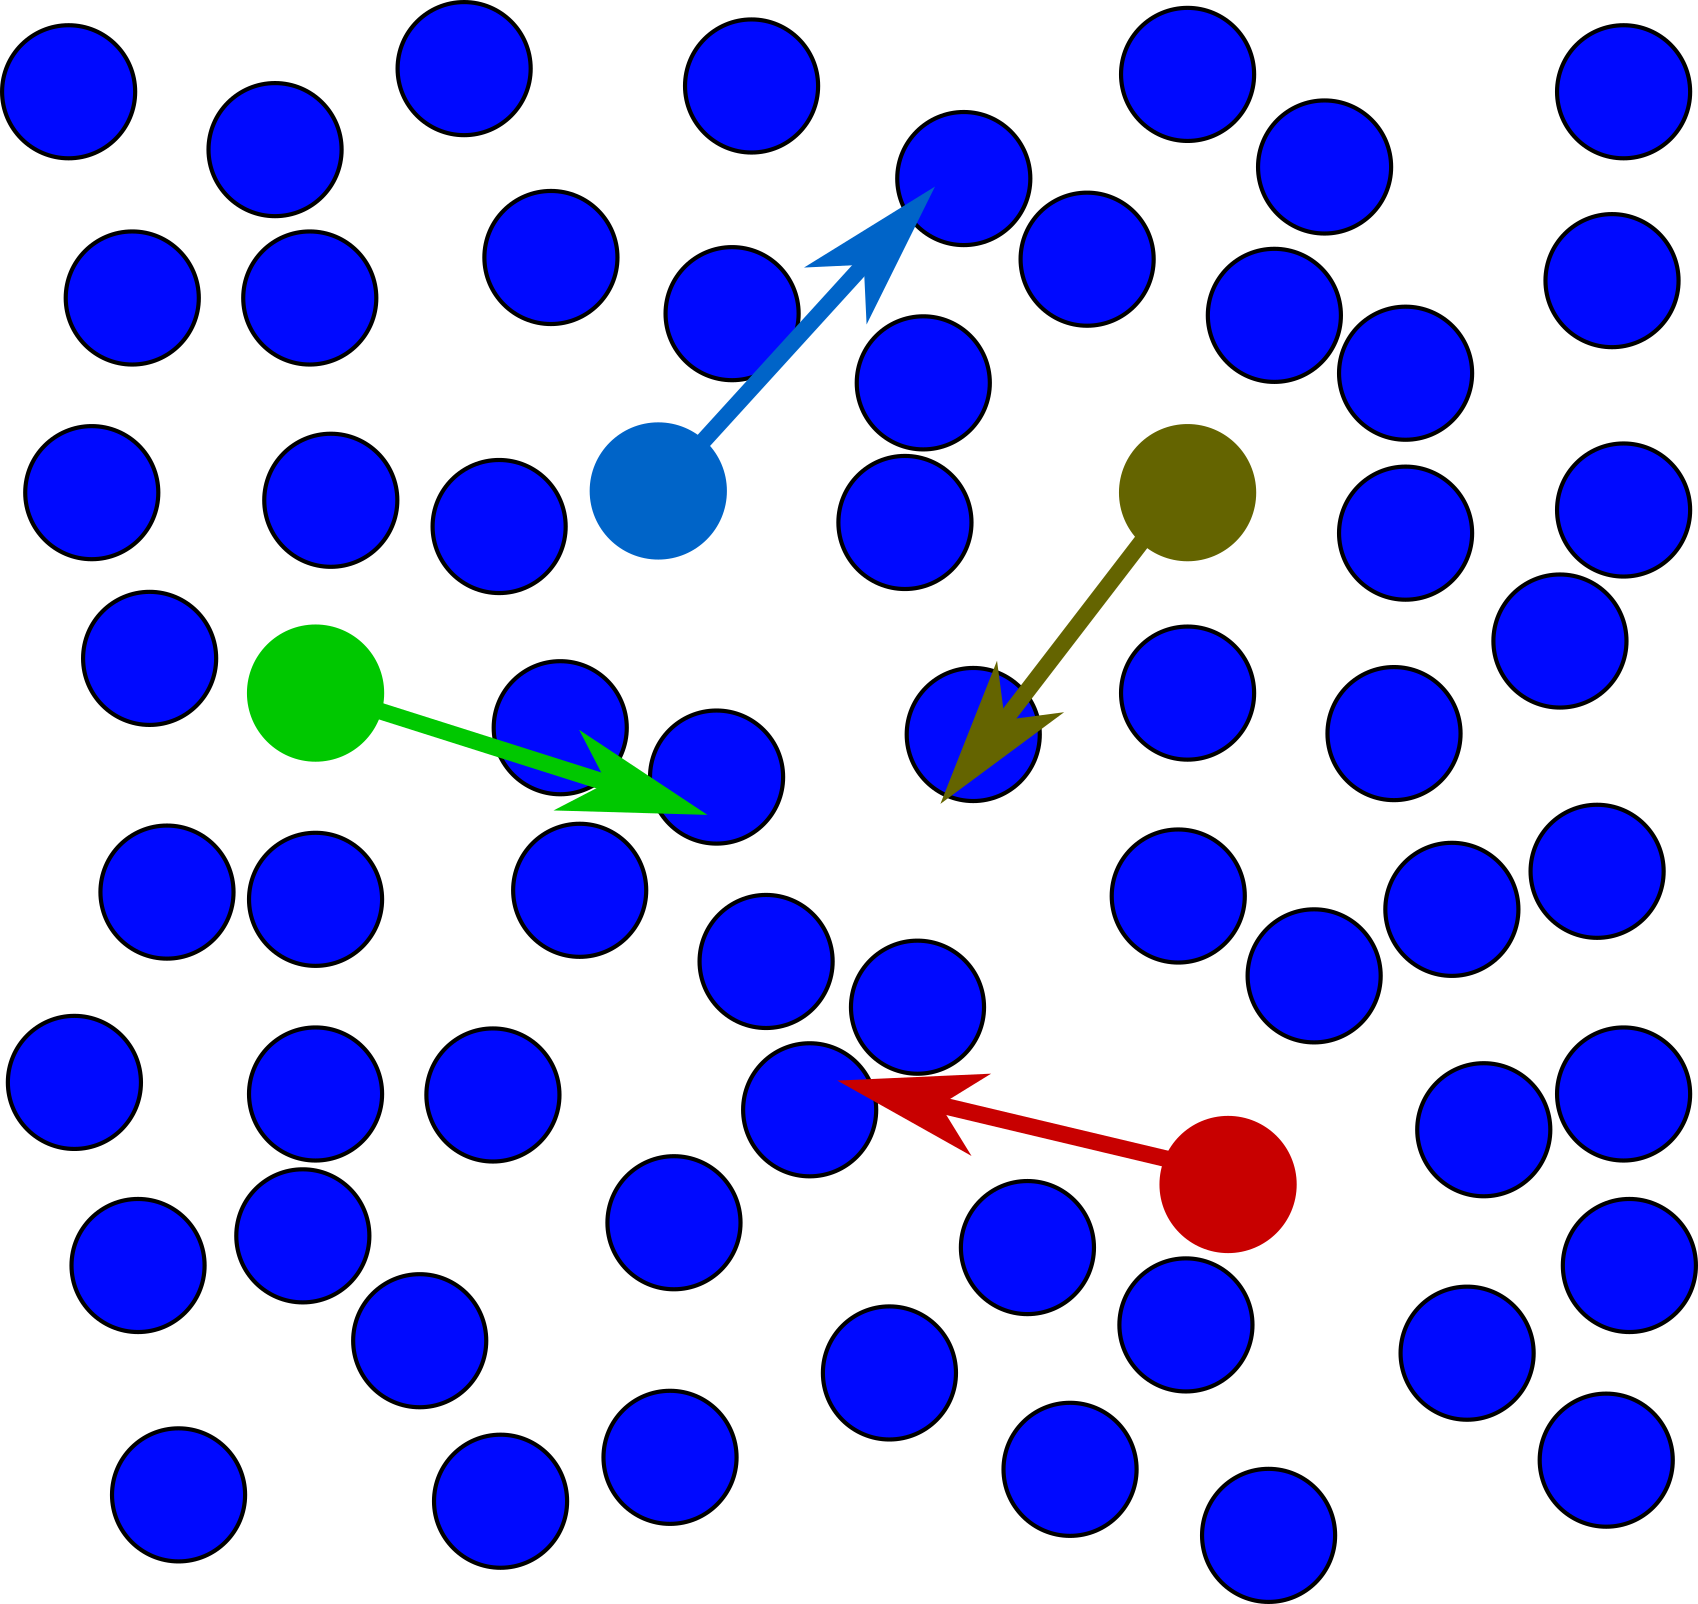
\includegraphics[width=.8\textwidth]{liquid_model_2.png}
						\end{center}
					\end{minipage}
				\end{center}

			\qitem 固体と液体の境目は?
				\begin{center}
					\begin{minipage}{0.44\textwidth}
						\begin{center}
						\begin{itembox}[l]{\qbox{}では固体的に}
							\begin{itemize}
								\item 流動するとは、
								\begin{itemize}
									\item 隙間に粒子が移動
									\item \qbox{}に他の粒子が移動
								\end{itemize}
								\item 粒子が動くより速く変形しようとすると?
								\begin{itemize}
									\item 速い速度で水を変形\\(高所から飛び込み)
									\item 液体が固体的な挙動
								\end{itemize}
							\end{itemize}
						\end{itembox}
						
\includegraphics[width=.32\textwidth]{dive.png}
						\end{center}
					\end{minipage}
					\begin{minipage}{0.42\textwidth}
						\begin{center}
						\begin{itembox}[l]{長時間では\qbox{}に}
							\begin{itemize}
								\item 長時間では氷河も流れる
								
								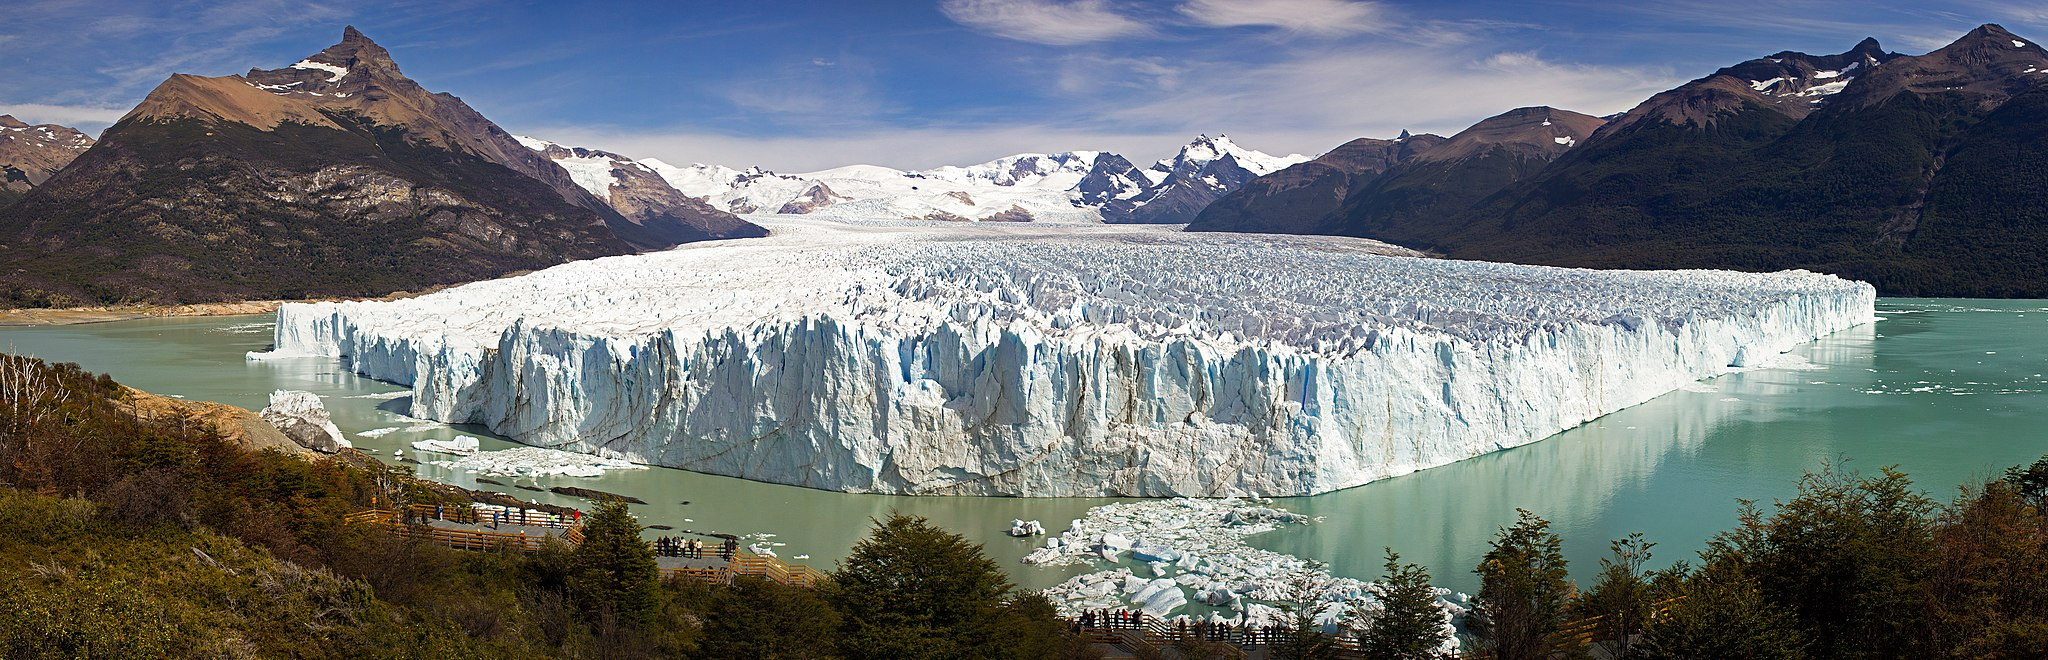
\includegraphics[width=.8\textwidth]{hyoga.jpg}
								\item コールタールも漏斗から\\流れ落ちる	
								
								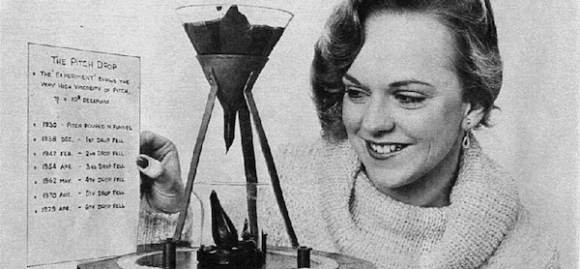
\includegraphics[width=.8\textwidth]{pitchdrop.png}
							\end{itemize}
						\end{itembox}
						\end{center}
					\end{minipage}
				\end{center}
				
			\qitem ガラス状態について
				\begin{center}
					\begin{minipage}{0.46\textwidth}
						\begin{itembox}[l]{ガラス状態}
							\begin{itemize}
								\item 液体からの冷却で、
								\item 常に\qbox{}するとは限らない。
								\begin{itemize}
									\item 非晶体:\qbox{}
									\item 流れない
									\item 例えば、\qbox{}等
								\end{itemize}
							\end{itemize}
						\end{itembox}
					\end{minipage}
					\begin{minipage}{0.4\textwidth}
						\begin{center}
						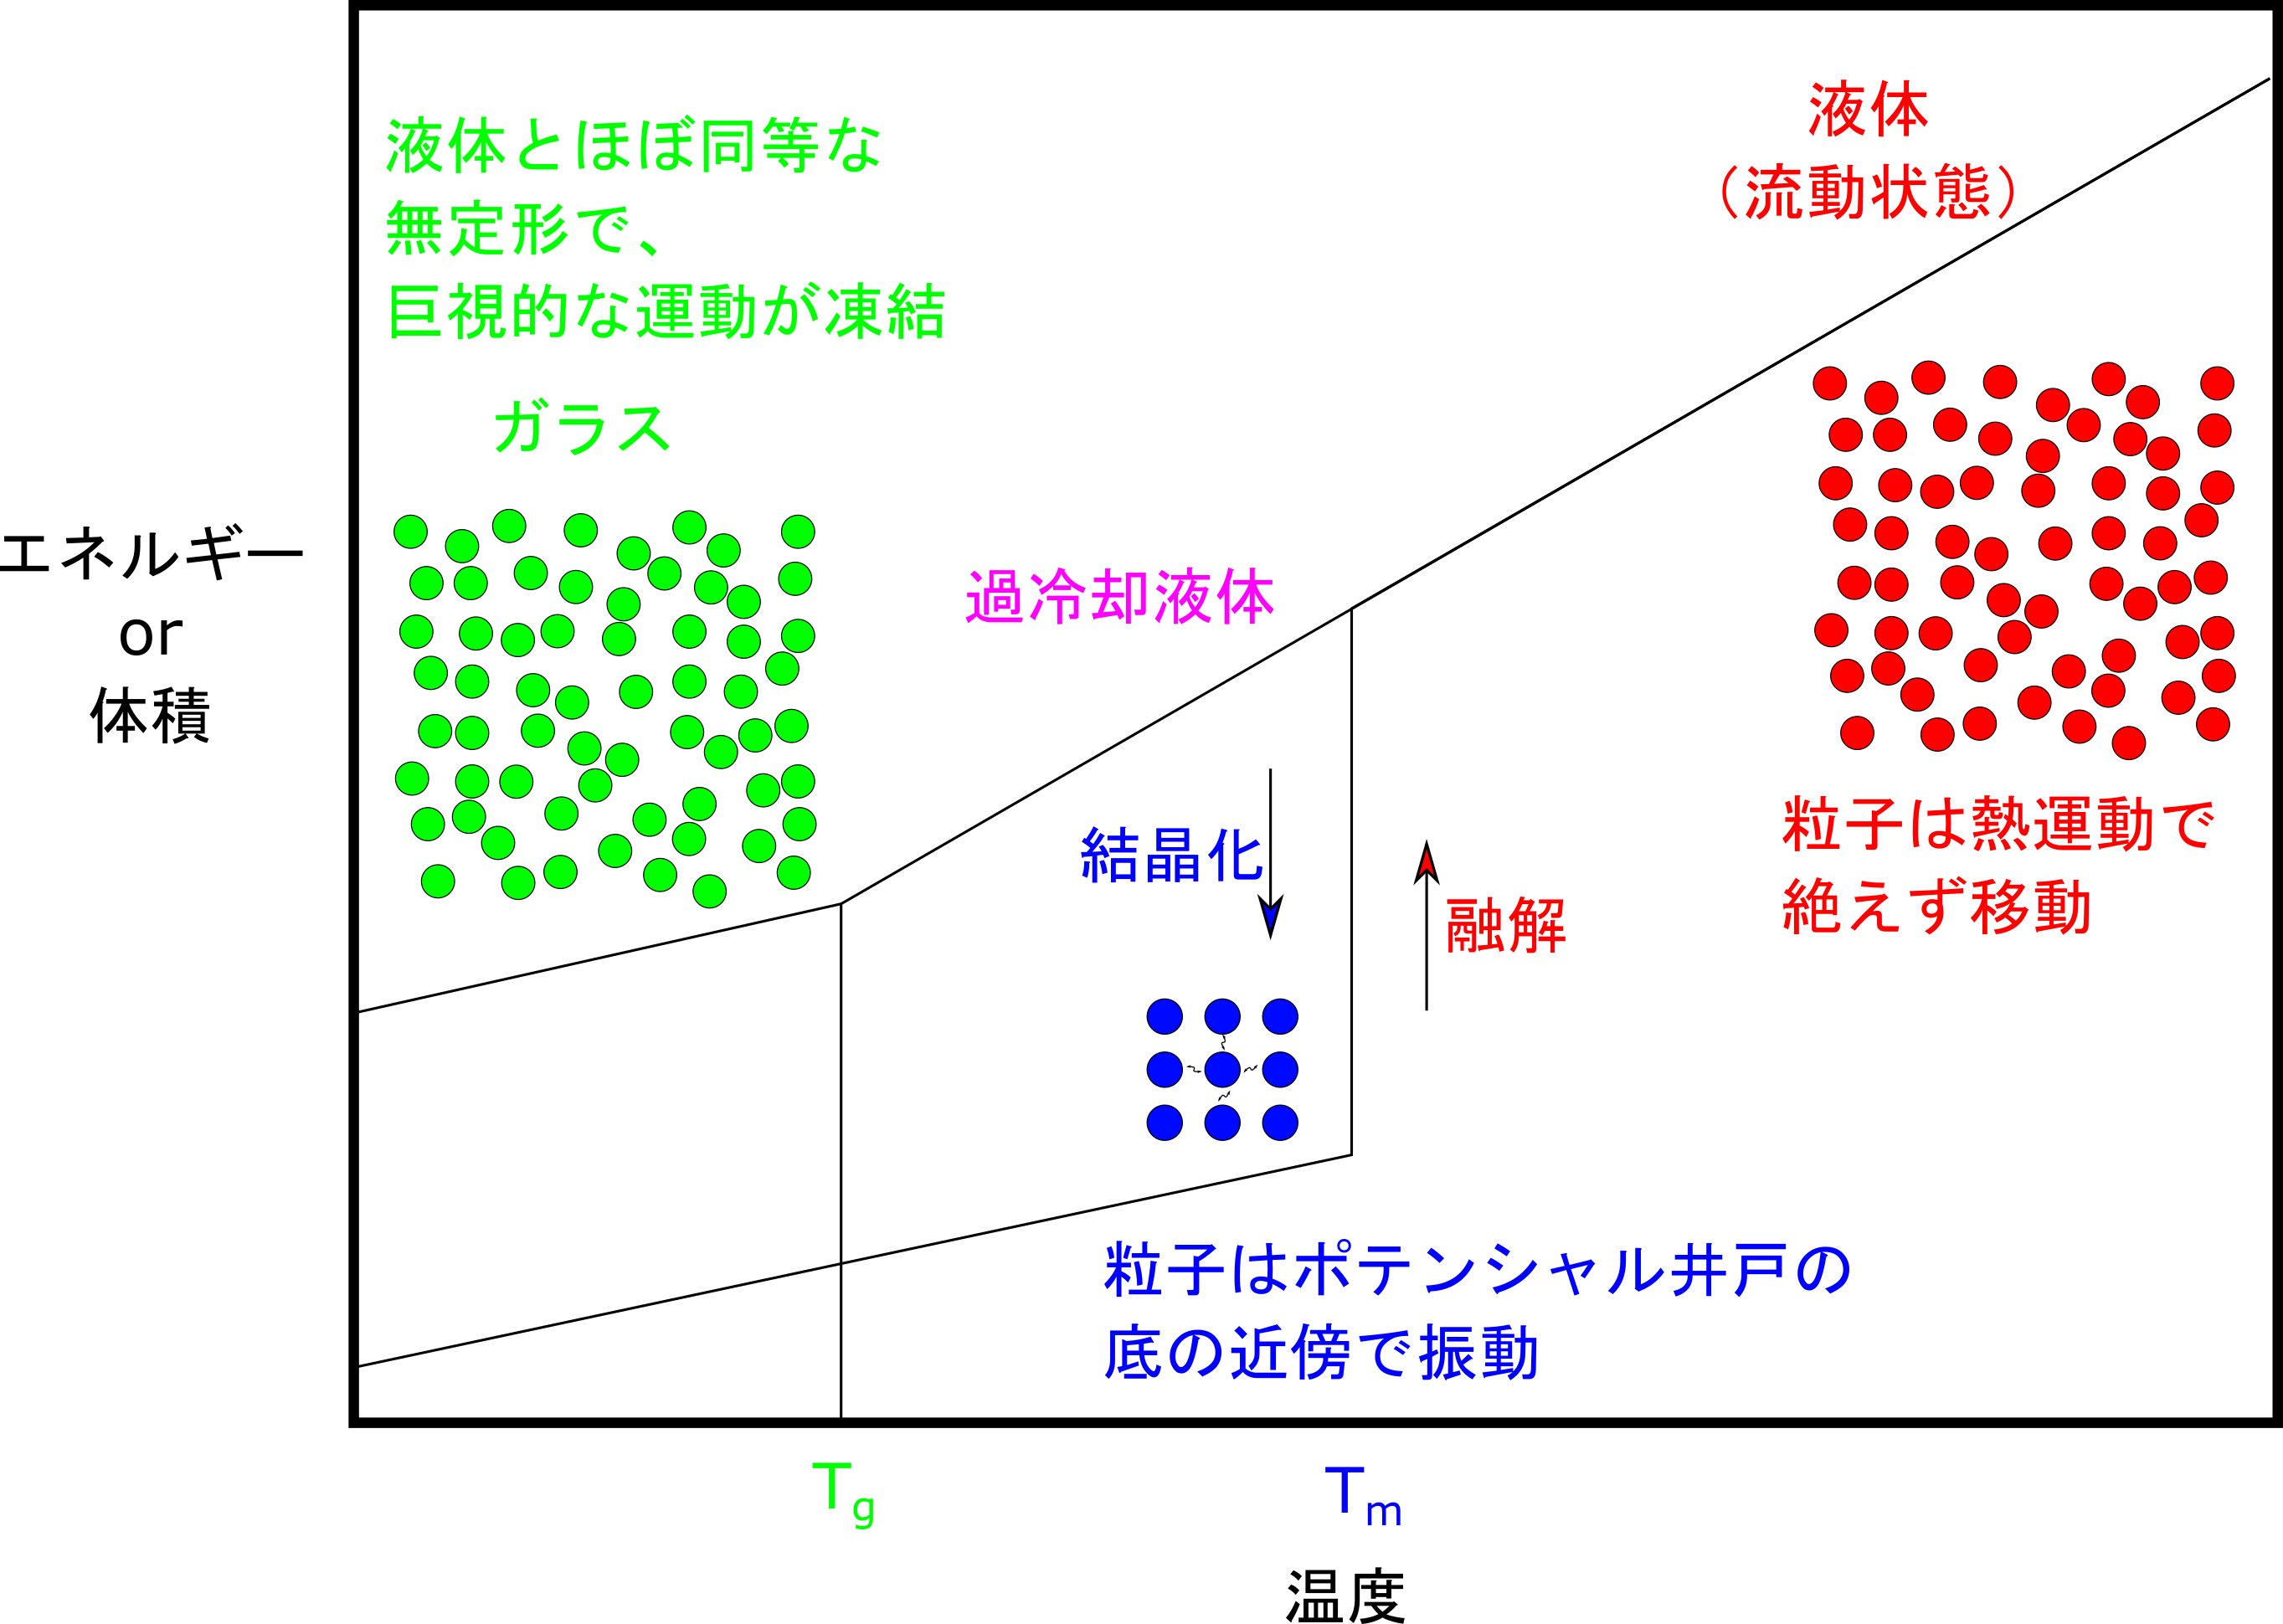
\includegraphics[width=\textwidth]{glass_trans.png}
						\end{center}
					\end{minipage}
				\end{center}
		\end{qlist2}

		\begin{itembox}[l]{選択肢}
			\begin{center}
				\begin{tabular}{lllll}
					1. 窓ガラス	&2. 再配置	&3. 液体的	&4. 最適化	&5. 速い変形\\
					6. アモルファス	&7. 結晶化		&8. 居心地が悪い	&9. 空いた場所
				\end{tabular}
			\end{center}
		\end{itembox}
\end{qlist}

\begin{itembox}[l]{解答}
    \begin{center} 
      \begin{tabular}{|c|c|c|c|c|c|c|c|c|} \hline
        (j) & (k) & (l) & (m) & (n) & (o) & (p) & (q) & (r)\\ \hline
         8  &  2 & 4 & 5 & 9 & 3 & 7 & 6 & 1 \\ \hline		
      \end{tabular}
    \end{center}
\end{itembox}


\begin{qlist}
	\qitem 「応力の起源」について、\qbox{(s)}から\qbox{(z)}までのカッコを埋めてください。
		\begin{qlist2}
			\qitem 結晶の応力の起源について
				\begin{center}
					\begin{minipage}{0.42\textwidth}
						\begin{itembox}[l]{マクロな変形の付与により}
							\begin{itemize}
								\item 固体内部でもミクロに変形
								\item マクロと相似に変形と単純化
								\item 粒子間で\qbox{}から変位
							\end{itemize}
						\end{itembox}
						\begin{center}
							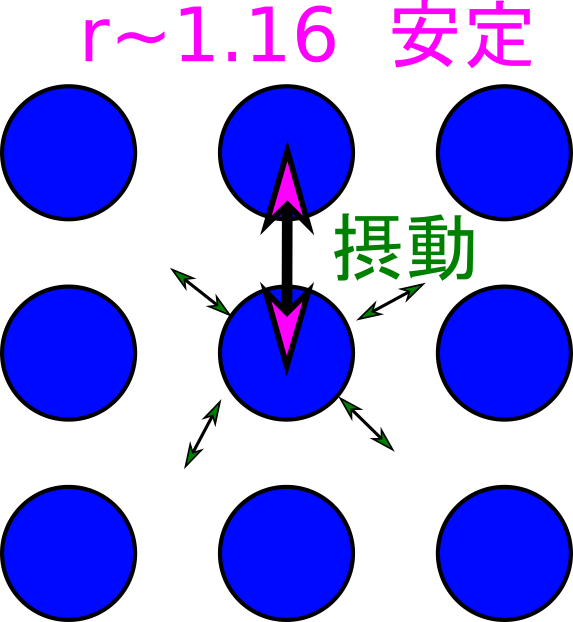
\includegraphics[width=.5\textwidth]{LJ_ryusi.png}
						\end{center}
					\end{minipage}
					\begin{minipage}{0.42\textwidth}
						\begin{itembox}[l]{ミクロに安定な位置から変位}
							\begin{itemize}
								\item 局所的には二体間で考えると、
								\begin{itemize}
									\item 接近した場合は、 $\Leftrightarrow$ 斥力
									\item 離反した場合は、 $\Leftrightarrow$ 引力
								\end{itemize}
								\item その\qbox{}として、マクロな応力が発生
							\end{itemize}
						\end{itembox}
						\begin{center}
							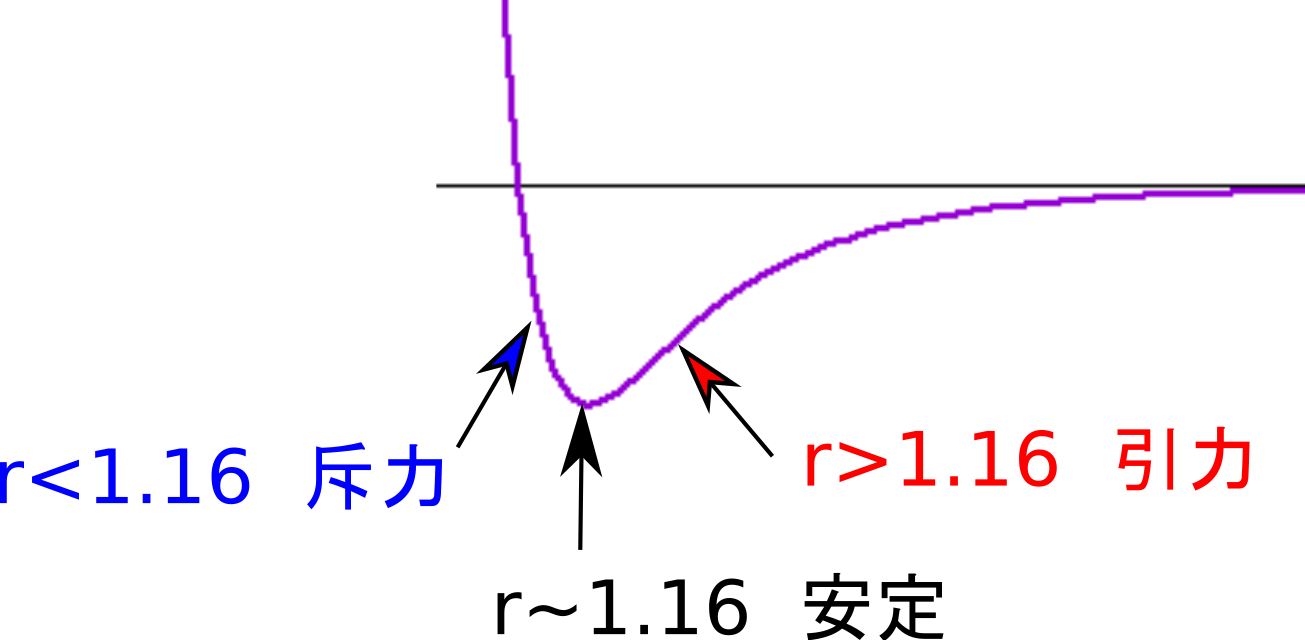
\includegraphics[width=\textwidth]{LJ_pos.png}
						\end{center}
					\end{minipage}
				\end{center}

			\qitem 固体と液体の違い
				\begin{itembox}[l]{固体と液体の違い}
					\begin{itemize}
						\item 固体では
						\begin{itemize}
							\item 単純な固体は一様に変形すると考えて、
							\item 生じる応力が一様で\qbox{}
						\end{itemize}
						\item 液体の場合
						\begin{itemize}
							\item 変形を止めれば、応力も\qbox{}すると考える。
							\item このとき、液体内部では、
							\begin{itemize}
								\item 粒子同士の相互作用が増加
								\item 粒子が\qbox{}すれば、増加分が消失
							\end{itemize}
						\end{itemize}
					\end{itemize}
				\end{itembox}
				
			\qitem 液体の応力について
				\begin{center}
					\begin{minipage}{0.42\textwidth}
						\begin{itembox}[l]{マクロな変形}
							\begin{itemize}
								\item マクロにせん断変形を付与
								\begin{itemize}
									\item ミクロにも粒子近傍が変形
								\end{itemize}
								\item 一粒子に着目すると、
								\begin{itemize}
									\item ポテンシャル場が変化
									\item 局所的に「\qbox{}」
								\end{itemize}
							\end{itemize}
						\end{itembox}
						\begin{center}
							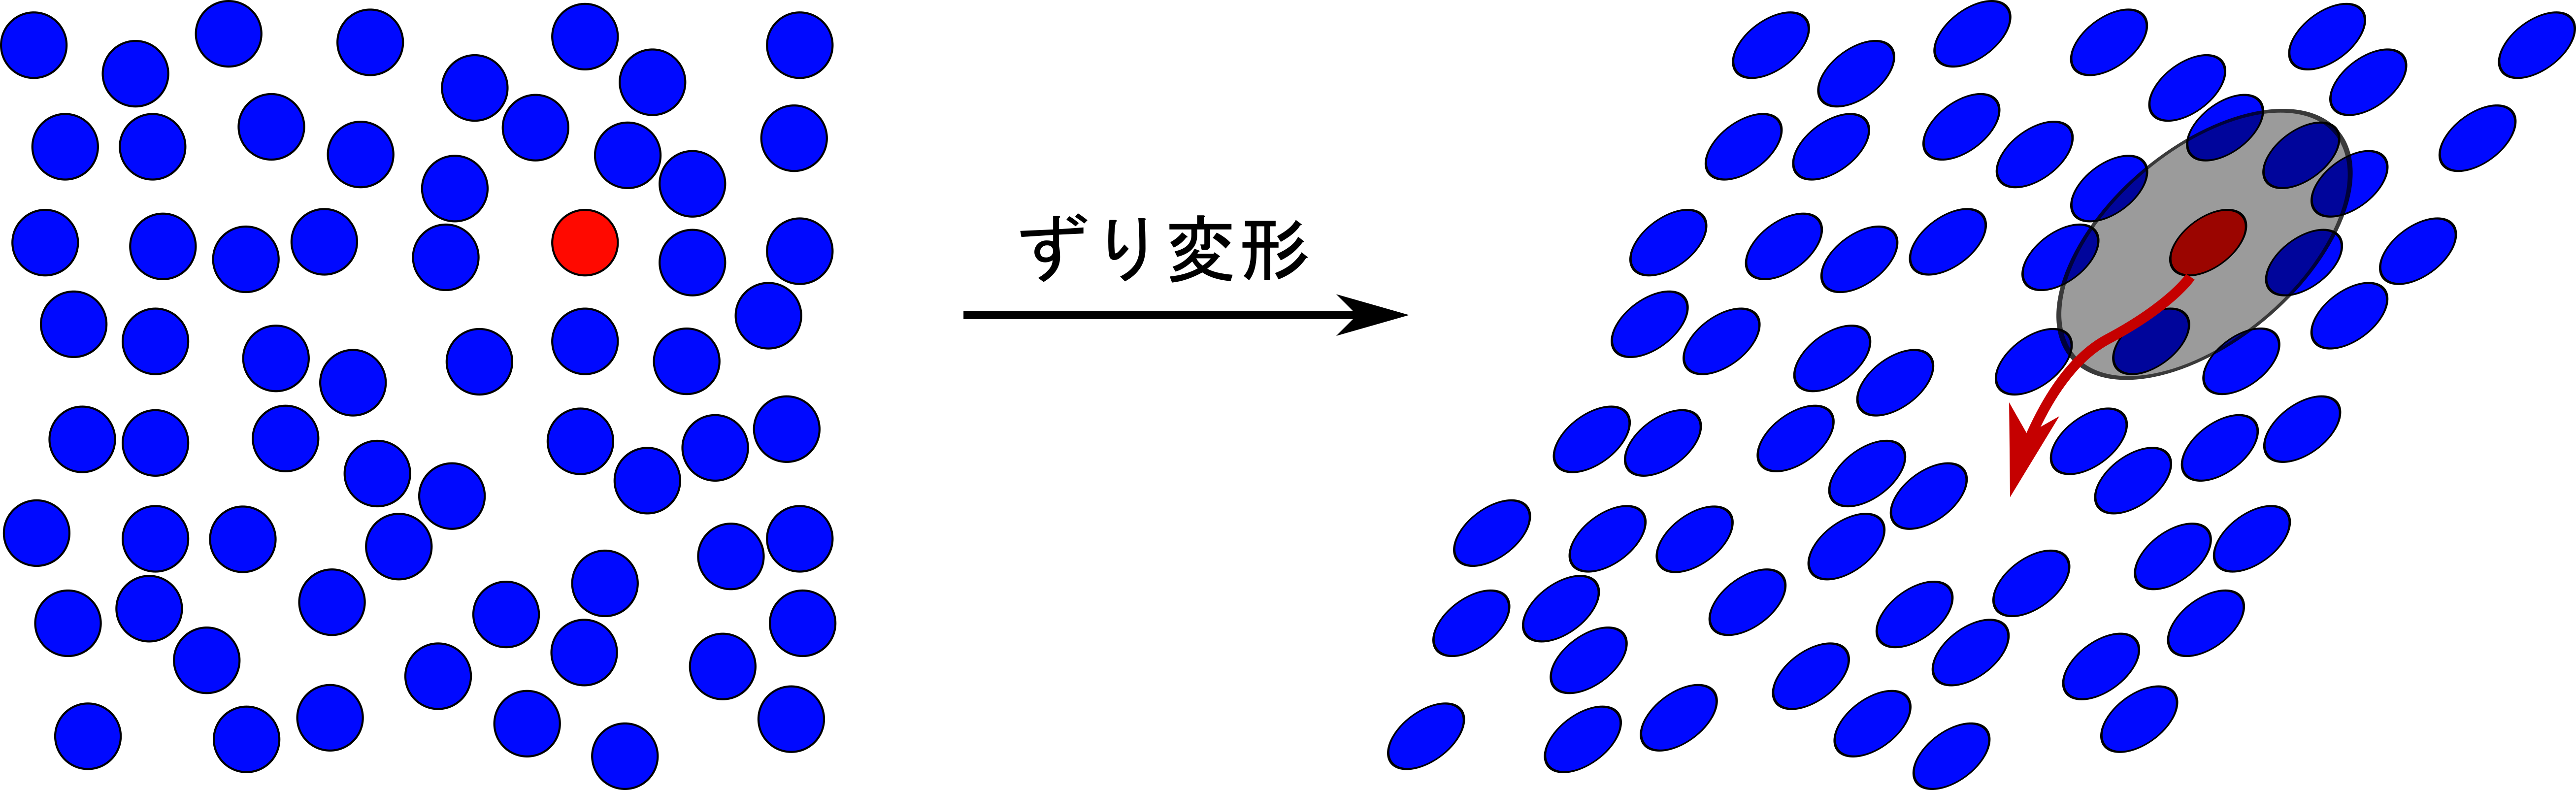
\includegraphics[width=.9\textwidth]{liquid_flow.png}
						\end{center}
					\end{minipage}
					\begin{minipage}{0.42\textwidth}
						\begin{itembox}[l]{ミクロな応力から流動へ}
							\begin{itemize}
								\item 「歪んだかご」の結果、
								\begin{itemize}
									\item 粒子の\qbox{}が悪化
									\item 局所的な応力が発現
									\item 積分値としてマクロな応力
								\end{itemize}
								\item 「歪んだかご」からの脱出
								\begin{itemize}
									\item ミクロな応力が消失
								\end{itemize}
								\item マクロにも\qbox{}
								\begin{itemize}
									\item マクロな応力も消失
								\end{itemize}
							\end{itemize}
						\end{itembox}
					\end{minipage}
				\end{center}
		\end{qlist2}

		\begin{itembox}[l]{選択肢}
			\begin{center}
				\begin{tabular}{lllll}
					1. 移動	&2. 居心地 	&3. 消失	&4. 積分値	&5. 持続的\\
					6. 流動	&7. 歪んだかご &8. 安定位置
				\end{tabular}
			\end{center}
		\end{itembox}
\end{qlist}

\begin{itembox}[l]{解答}
    \begin{center} 
      \begin{tabular}{|c|c|c|c|c|c|c|c|} \hline
        (s) & (t) & (u) & (v) & (w) & (x) & (y) & (z) \\ \hline
        8 & 4 & 5 & 3 & 1 & 7 & 2 & 6 \\ \hline		
      \end{tabular}
    \end{center}
\end{itembox}

\clearpage

\question{演習問題 3}
説明文中の言葉を使って数行程度の簡単な記述で構いませんので、以下の自由記述問題を考えてみてください。
\begin{qlist}
\qitem この章では、物理化学として物質を見直すという観点で、固体と液体の違いについてミクロなイメージの説明を行いました。

レオロジーという学問においては、流れるということが最も重要な現象となりますので、
文中の言葉をそのまま使って結構ですから、ご自分なりの「流れるとはどういう現象なのか」ということを書いてみてください。
\end{qlist}

\begin{itembox}[l]{解答例}
    流れるという現象は、マクロに与えた変形等の刺激に対して、液体がその形を変えることによって、与えられた刺激をなかったことにしていく過程と考えることができます。
	% なお、変形を与えている間は、その変形速度に比例する形で移動(流れ)を止めようとする応力が発生する。

	この現象をミクロに見ると、物質の内部ではもともと粒子はあらゆる方向(等方的:どの方向も平等)に移動しており、これは拡散現象と呼ばれます。
	マクロな変形により異方的(特定の方向にエコヒイキ)に粒子の居心地が悪くなった際に、それを改善するためにミクロな物質の移動が生じていると考えることが出来ます。
\end{itembox}

\clearpage

\end{document}